\documentclass[fleqn]{article}
\usepackage[english]{babel}
\usepackage{amsmath}
\usepackage{amsthm}
\usepackage{graphicx}
\usepackage[utf8]{inputenc}

%%%%%%%% MARGIN
\usepackage[left=1in, right=1in, top=0.8in, bottom=0.8in]{geometry}

%%%%%%%% NO PARAGRAPH INDENT
% https://tex.stackexchange.com/questions/27802/set-noindent-for-entire-file
\setlength\parindent{0pt}

%%%%%%%% SUB-FIGURE PACKAGE
\usepackage{subcaption}

\usepackage{pdfpages}

%%%%%%%% HYPERREF PACKAGE
\usepackage{hyperref}
\hypersetup{linkcolor=blue}
\hypersetup{citecolor=blue}
\hypersetup{urlcolor=blue}
\hypersetup{colorlinks=true}

%%%%%%%% MULTI-COLUMNS PACKAGE
\usepackage{multicol}

%%%%%%%% SETS DEFINITIONS
\usepackage{amssymb}
%%%% Important sets
\renewcommand{\O}{\mathbb{O}}
\newcommand{\N}{\mathbb{N}}
\newcommand{\Z}{{\mathbb{Z}}}
\newcommand{\Q}{{\mathbb{Q}}}
\newcommand{\RR}{{\mathbb{R}}}

%%%% Statistics
\newcommand{\E}[1]{\mathbb{E}\left[#1 \right]}
\newcommand{\V}[1]{\mathbb{V}\left[#1 \right]}
\newcommand{\cov}[1]{\mathrm{Cov}\left[#1 \right]}

%%% Misc Math
% Spaces after/before left/right
\let\originalleft\left
\let\originalright\right
\renewcommand{\left}{\mathopen{}\mathclose\bgroup\originalleft}
\renewcommand{\right}{\aftergroup\egroup\originalright}

% Norm and abs
\newcommand{\norm}[1]{\left\lVert#1\right\rVert}
\newcommand{\abs}[1]{\left\lvert#1\right\rvert}

%%%% Superscript to the left
% https://latex.org/forum/viewtopic.php?t=455
\usepackage{tensor}
\newcommand{\app}[3]{\tensor*[^{#1}]{\left(#2, #3\right)}{}}


%%%%%%%% SPLIT EQUATIONS
% https://tex.stackexchange.com/questions/51682/is-it-possible-to-pagebreak-aligned-equations
\allowdisplaybreaks

%%%%%%%% CODE RENDERING
% Compile with flag -shell-escape
\usepackage{minted}

%%%%%%%% EXAM PACKAGE
\usepackage{mathexam}

%%%%%%%% CHANGE MARGINS ITEMIZE
\usepackage{enumitem}

%%%%%%%% START DOCUMENT

\ExamClass{EC0301 - Time Series}
\ExamName{Assignment \#7}
\ExamHead{\today}

\let\ds\displaystyle

\begin{document}
 \vspace{0.3cm}
   % Information of the student
   \begin{itemize}[leftmargin=6.25cm, labelsep=0.5cm]

     \item[\textit{Name}] \scalebox{1.2}{David Plazas Escudero} % Name
     \item[\textit{Student code}] 201710005101 % Code

   \end{itemize}
\vspace{0.3cm}

% Each of the items to solve
\begin{enumerate}
\item \textit{Calculate the first five predictions and the associated MSE to these predictions, for an ARMA(2,1) model.}
\begin{figure}[H]
    \centering
    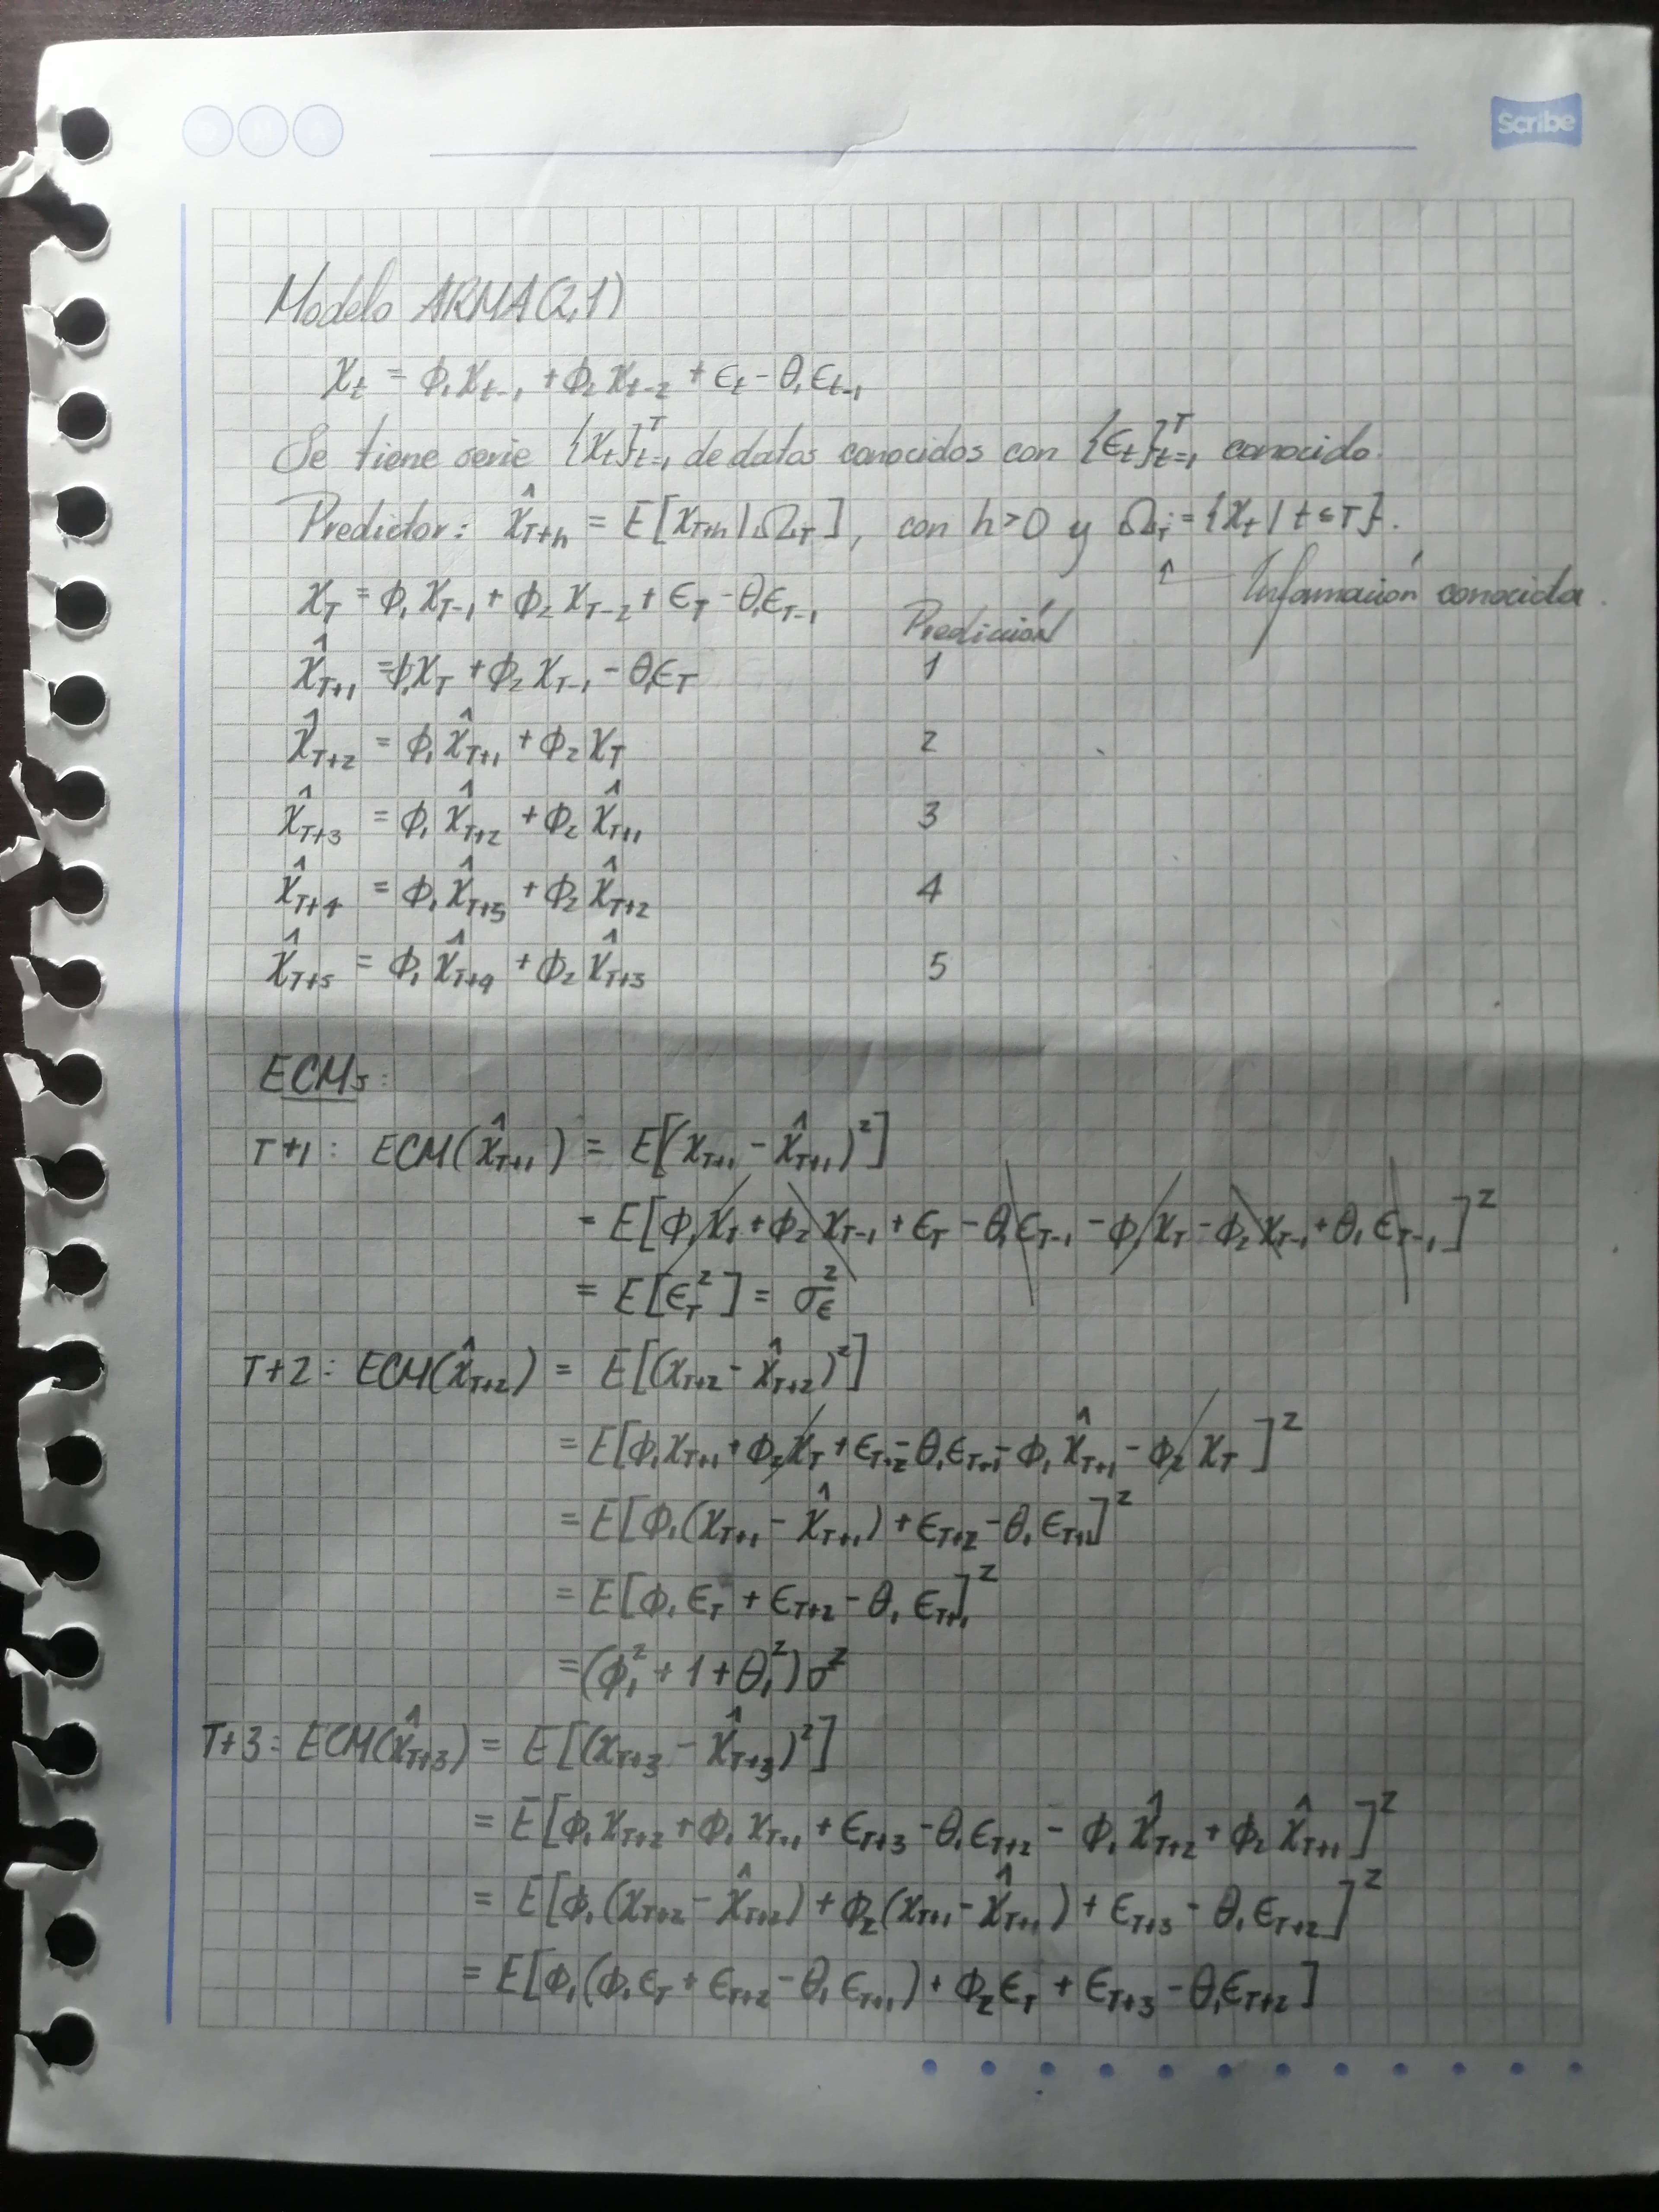
\includegraphics[width=0.8\linewidth]{figs/11.jpg}
\end{figure}
\begin{figure}[H]
    \centering
    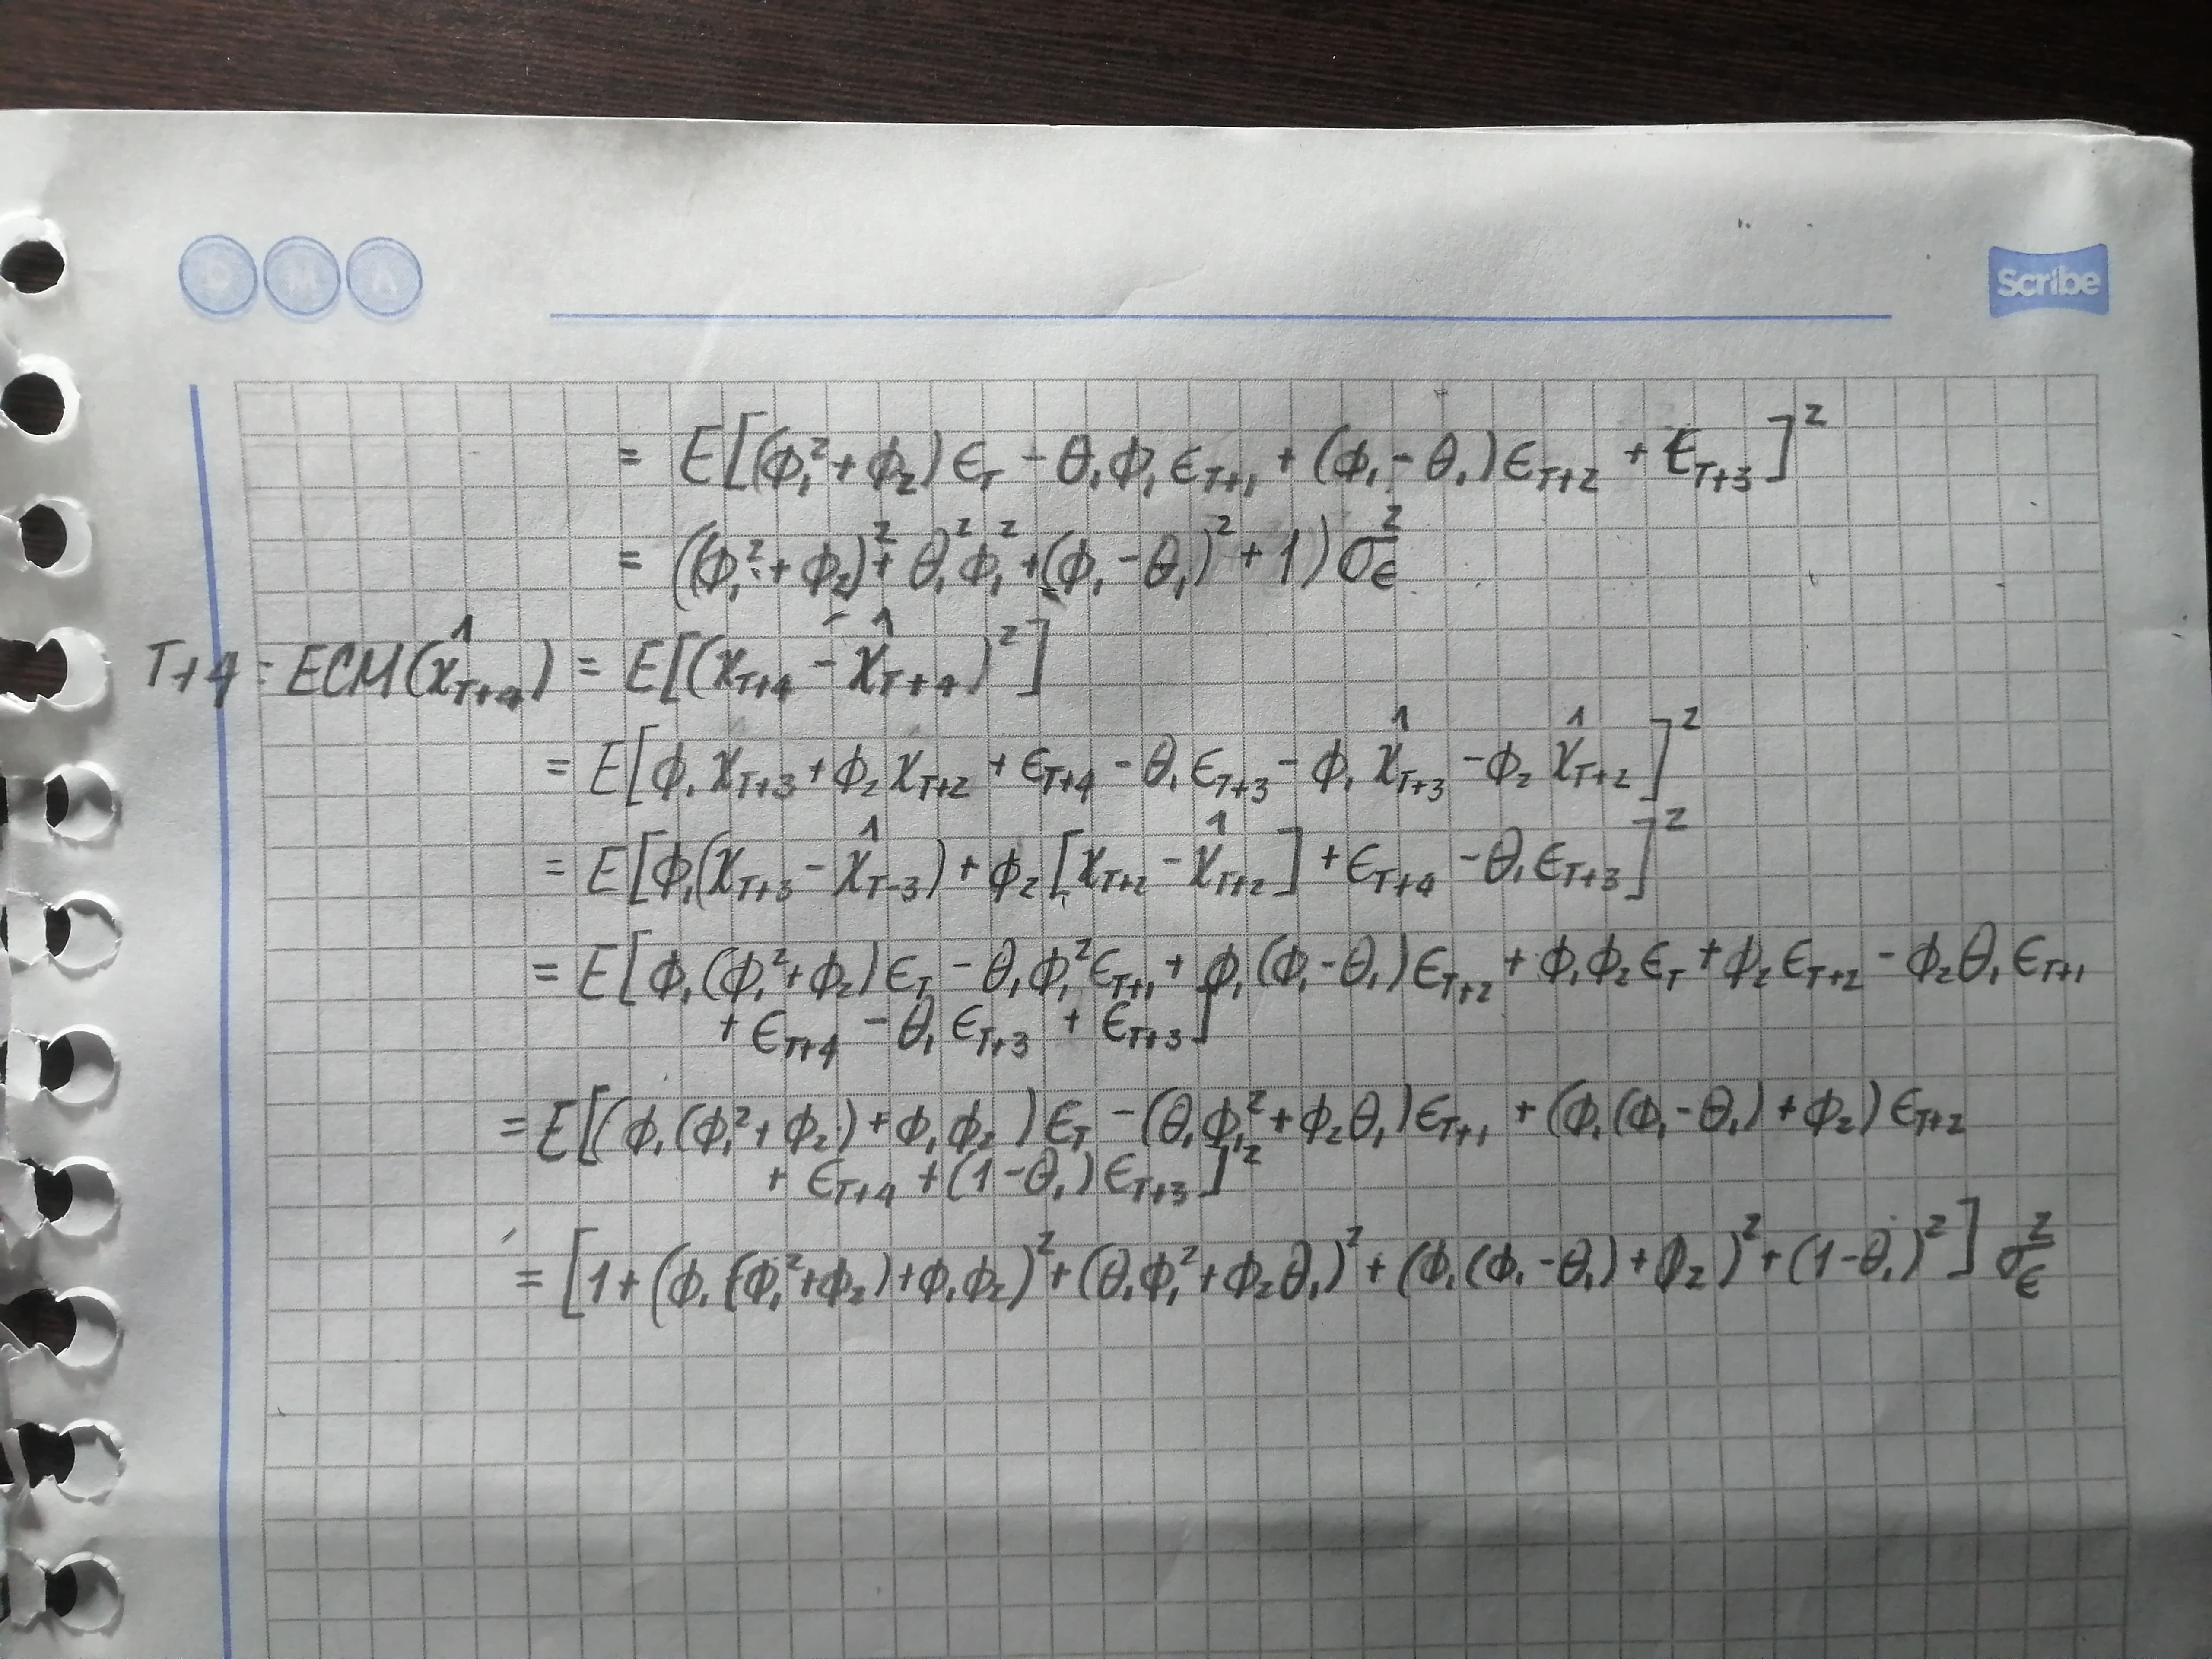
\includegraphics[width=0.8\linewidth]{figs/12.jpg}
\end{figure}
\item{\textit{Show that the MSE of the conditional expectation is the variance of the prediction error.}}

Let $\{Y_t\}_{t=1}^T$ be the time series data. Let $\{\hat{Y}_{T+h}\}_{h>0}$ be the predicted values for the series data for $t>T$, calculated by the conditional expectation predictor: $\hat{Y}_{T+h}=\E{Y_{T+h}|\,\Omega_T}$. 

Let us prove that $\hat{Y}_{T+h}$ is an unbiased estimator of $Y_{T+h}$: let $B[\hat{\theta}]$ be the bias of the estimator $\hat{\theta}$ of a parameter $\theta$. Hence, in our case
\[
B\left[\hat{Y}_{T+h}\right]=\E{Y_{T+h}-\E{Y_{T+h}|\,\Omega_T}},
\]
since $\E{\cdot}$ is linear operator
\[
B\left[\hat{Y}_{T+h}\right]=\E{Y_{T+h}}-\E{\E{Y_{T+h}|\,\Omega_T}},
\]
and by law of iterated expectations,
\[
B\left[\hat{Y}_{T+h}\right]=\E{Y_{T+h}}-\E{Y_{T+h}}=0.
\]
Thus, $\hat{Y}_{T+h}$ is an unbiased estimator of $Y_{T+h}$. Now, the variance of the prediction error is
\[
\V{Y_{T+h}-\hat{Y}_{T+h}}=\E{\left(Y_{T+h}-\hat{Y}_{T+h}\right)^2}-\mathbb{E}^2\left[Y_{T+h}-\hat{Y}_{T+h}\right],
\]
and since $\hat{Y}_{T+h}$ is an unbiased estimator of $Y_{T+h}$, the right-most term is zero. Then
\[
\V{Y_{T+h}-\hat{Y}_{T+h}}=\E{\left(Y_{T+h}-\hat{Y}_{T+h}\right)^2}=\mathrm{MSE}\left[\hat{Y}_{T+h}\right]
\]
\item{\textit{Estimate an ARIMA model using the data from Assignment 5, by minimizing an chosen information criterion (AIC or BIC) and validate if the estimated model satisfy the validation requirements.}}
One by one, the validation requirements will be covered:
\begin{itemize}
    \item \textbf{White noise residuals:} the estimated mean of the series is 0.005. The plot of the time series' residuals is presented in Figure \ref{fig:res}. It can be observed that the variance of the residuals is constant over time.
    \begin{minted}{r}
    library(readr)
    library(forecast)
    library(tseries)
    
    data <- read.csv("data.csv")
    data <- data[2]
    attach(data)
    x <- as.ts(data)
    
    fit = auto.arima(data, ic="aic")
    ts.plot(fit[["residuals"]])
    \end{minted}
    \begin{figure}[H]
        \centering
        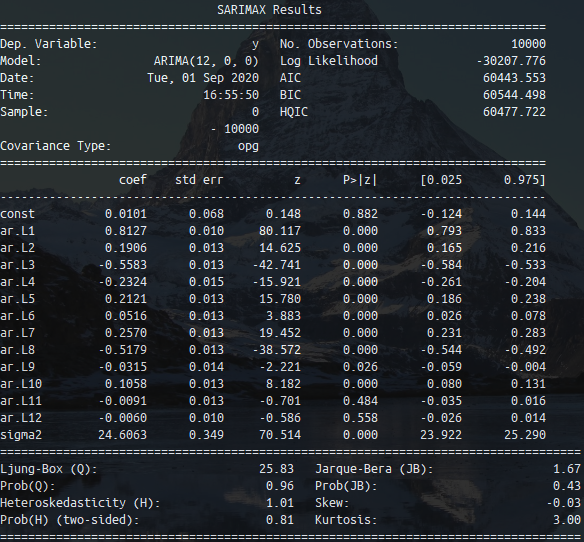
\includegraphics[scale=0.4]{res.png}
        \caption{Residuals}
        \label{fig:res}
    \end{figure}
    Finally, the autocorrelation and partial autocorrelation plots of the residuals are presented in Figure \ref{fig:acf}. It can be observed that the data is autocorrelated for several lags. This was also proved by the Box statistic: a p-value of $2.2\times10^{-16}$ means that the null hypothesis shall be rejected and, thus, the residuals are autocorrelated.
    
    \begin{minted}{r}
    acf(fit[["residuals"]])
    pacf(fit[["residuals"]])
    Box.test(x)
    \end{minted}
    
    \begin{figure}[H]
    \centering
    \begin{subfigure}[b]{\textwidth}
        \centering
        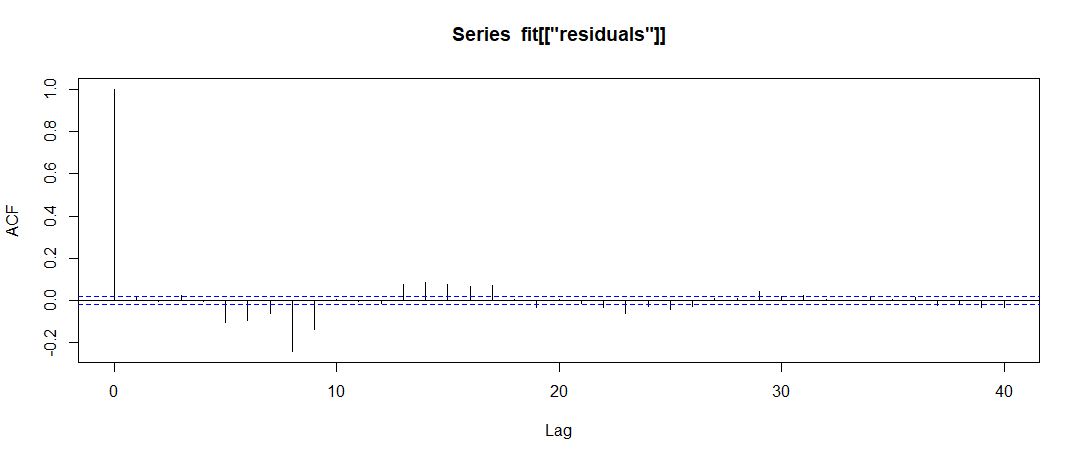
\includegraphics[scale=0.4]{figs/acf.png}
        \caption{Standard.}
    \end{subfigure}
    \begin{subfigure}[b]{\textwidth}  
        \centering 
        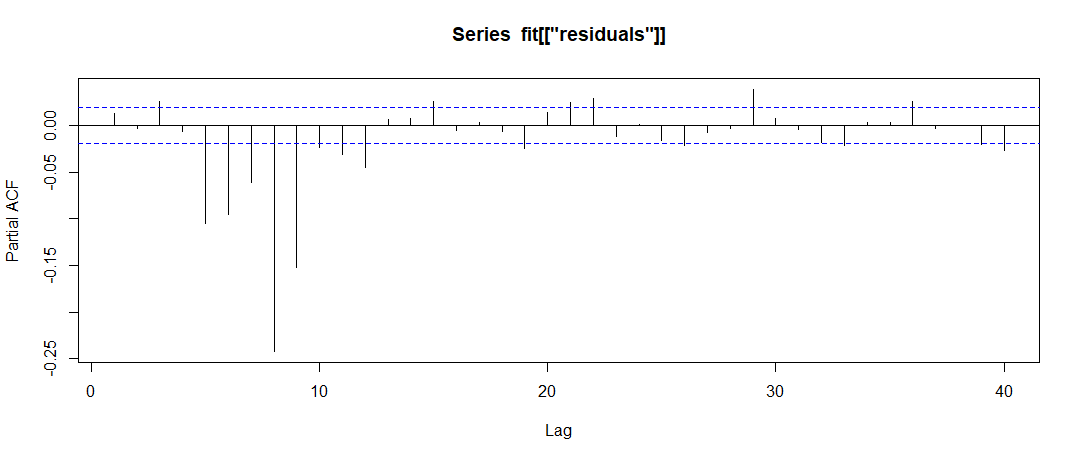
\includegraphics[scale=0.4]{figs/pacf.png}
        \caption{Partial.}
    \end{subfigure}]
    \caption{Autocorrelation plots.}
    \label{fig:acf}
\end{figure}
\item \textbf{Stationarity and invertibility:} The estimated model is both stationary and invertible, since all the roots, in both the AR and MA components, are inside the unit circle, as seen in Figure \ref{fig:roots}. Although, some of them are quite close to the boundary of the circle.
\begin{minted}{r}
    plot(fit)
\end{minted}
\begin{figure}[H]
    \centering
    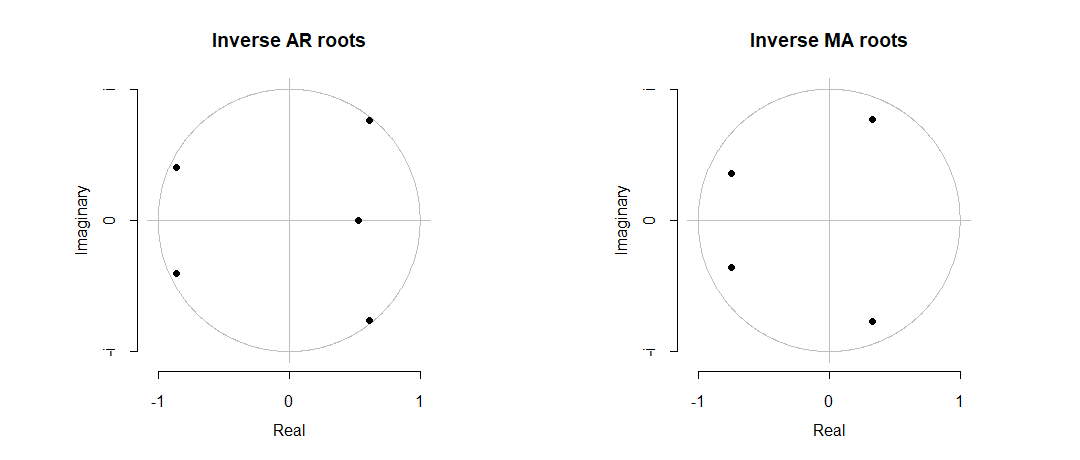
\includegraphics[scale=0.4]{figs/roots.png}
    \caption{Roots of estimated model.}
    \label{fig:roots}
\end{figure}
\item \textbf{Significative and non-correlated parameters:} The estimated correlation between the parameters is presented in the matrix in Figure \ref{fig:corr}. It can be observed that, in general, all parameters are highly correlated.
\begin{minted}{r}
    cov2cor(fit[["var.coef"]])
\end{minted}
\begin{figure}[H]
    \centering
    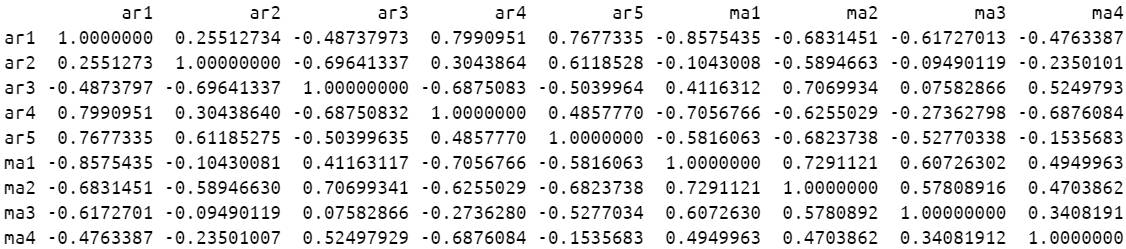
\includegraphics[scale=0.4]{figs/corr.png}
    \caption{Parameters correlation.}
    \label{fig:corr}
\end{figure}
\item \textbf{D.G.P. representation:} To test that the model adequately represents the D.G.P., the White test for linearity was used:
\begin{minted}{r}
    white.test(x)
\end{minted}
A p-value of 0.88 was obtained, and hence the null hypothesis of linearity is not rejected. There is evidence of linearity in the series data.
\item \textbf{Goodness of fit:} The estimated $R^2$ for the fitted model is 0.86, which is a relatively high $R^2$, and we conclude that the model correctly fits the time series data to a certain degree.
\begin{minted}{r}
    R2 = 1 - var(fit[["residuals"]])/var(x)
\end{minted}
\end{itemize}
In summary, the fitted ARIMA model does not satisfy the requirement of white noise; it does satisfy the invertibility and stationarity; it does not satisfy that the parameters are not correlated; it satisfy the hypothesis of linearity of the D.G.P.; and it fit adequately de time series data.
\end{enumerate}
\end{document}
